\chapter{Procedimiento experimental}

\section{Materiales utilizados}
\begin{itemize}
    \item Balanza granataria.
    \begin{itemize}
        \item Capacidad: 7 kilogramos.
        \item Precisión: 1 gramo.
    \end{itemize}
    \item Viga de madera con una cinta métrica graduada en milímetros.
    \item Tres baldes plásticos para colgar las masas.
    \item Cinta adhesiva.
    \item Masas de distintos valores.
\end{itemize}


A continuación se detallan las masas utilizadas a lo largo de la experiencia y sus pesos respectivos. Para calcular el peso ($F$), se multiplicó la masa experimental por la aceleración de gravedad estándar ($g \approx 9.8 \, \text{m/s}^2$).

\begin{itemize}
    \item \textbf{Primera Parte (Eje en Orificio A):}
    \begin{itemize}
        \item Masa 1 ($m_1$): $0.100$ kg $\rightarrow$ Peso $\approx 0.98$ N
        \item Masa 2 ($m_2$): $0.203$ kg $\rightarrow$ Peso $\approx 1.99$ N
        \item Masa 3 ($m_3$): Varía de $0.303$ a $0.564$ kg $\rightarrow$ Peso $\approx 2.97$ a $5.53$ N
    \end{itemize}
    \vspace{0.2cm}
    \item \textbf{Segunda Parte (Eje en Orificio B):}
    \begin{itemize}
        \item Masa 1 ($m_1$): $0.048$ kg $\rightarrow$ Peso $\approx 0.47$ N
        \item Masa 2 ($m_2$): $0.101$ kg $\rightarrow$ Peso $\approx 0.99$ N
        \item Masa 3 ($m_3$): $0.820$ kg $\rightarrow$ Peso $\approx 8.04$ N
    \end{itemize}
\end{itemize}

\newpage

\vspace{0.5cm}
\begin{figure}[H]
    \centering
    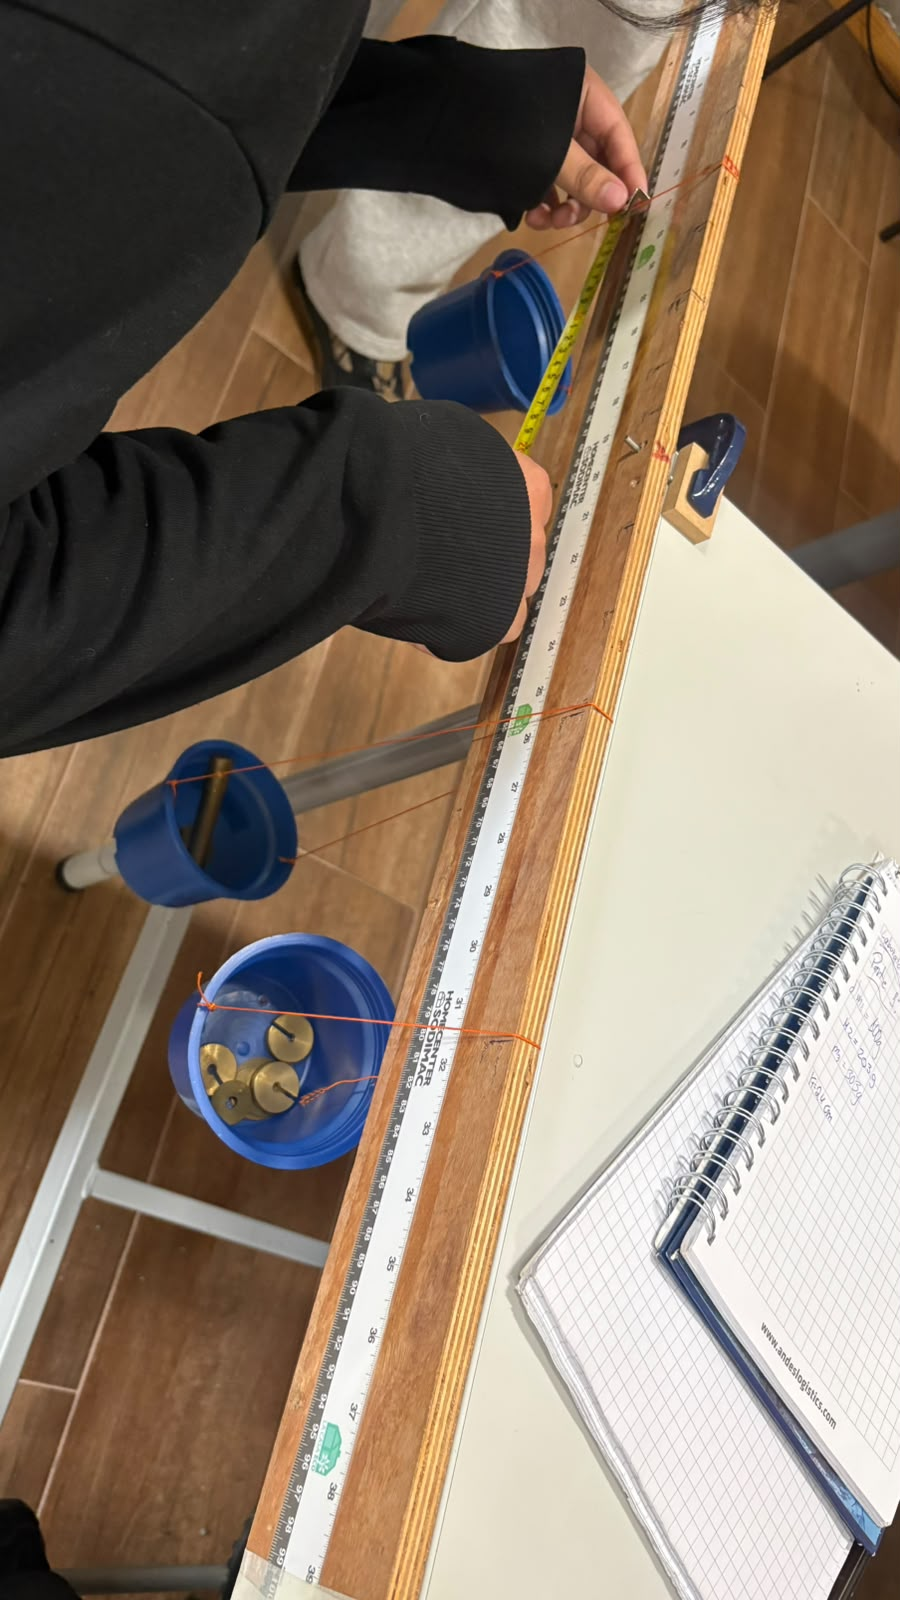
\includegraphics[angle=90, scale=0.25]{parte a.jpeg}
    \caption{Imagen del montaje de la Primera Parte.}
\end{figure}

\begin{figure}[H]
    \centering
    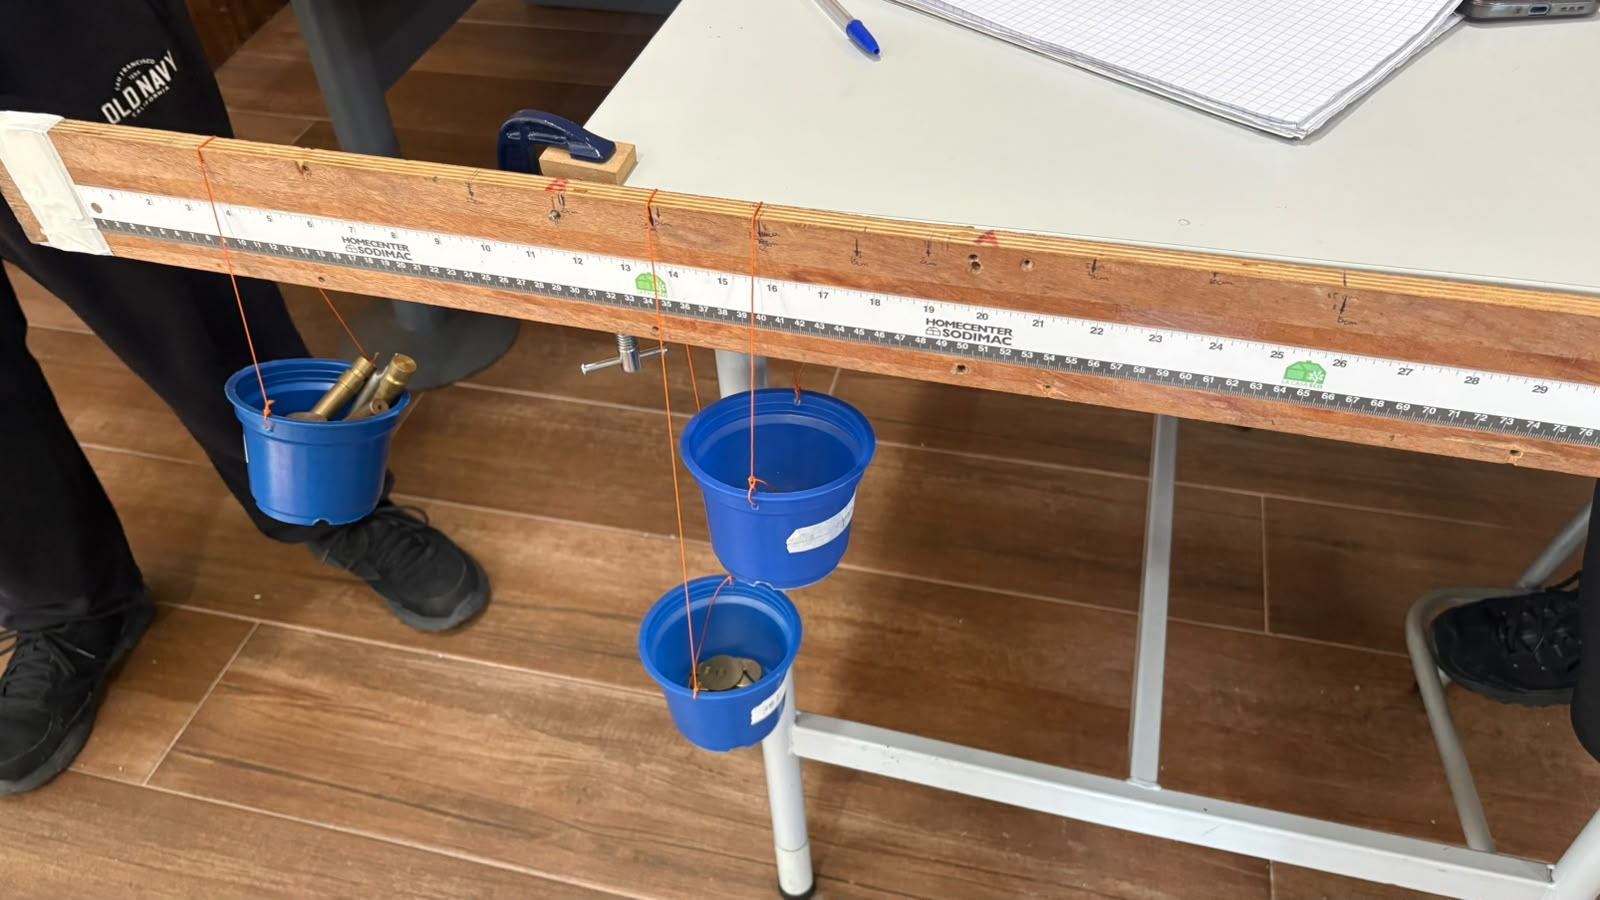
\includegraphics[scale=0.25]{parteb.jpeg}
    \caption{Imagen del montaje de la Segunda Parte.}
\end{figure}

\newpage

\section{Procedimiento}

Para el montaje y la realización del experimento, se siguieron los siguientes pasos:

\begin{enumerate}
    \item Se midió la masa de la viga, obteniéndose un valor aproximado de $770$ g.

    \item Se suspendió inicialmente la viga desde el orificio A y se observó que permanecía aproximadamente horizontal, debido a que este punto coincidía con su centro de masa.

    \item Se colocaron en cada recipiente las masas correspondientes a cada caso experimental.

    \item Una vez preparadas las masas, los recipientes se colgaron de la viga a las distancias indicadas para cada configuración.

    \item Con las masas $m_1$ y $m_2$ ubicadas en sus respectivas posiciones, se determinó la masa o la distancia necesaria para $m_3$, según correspondiera en cada caso, con el fin de mantener la viga en equilibrio.

    \item El procedimiento se repitió para los casos correspondientes al orificio A, modificando las masas y las distancias de acuerdo con cada configuración.

    \item Posteriormente, la viga se suspendió desde el orificio B y se repitió el procedimiento anterior. En esta configuración se consideró además el torque producido por el peso de la propia viga, debido a que el punto de suspensión no coincidía con su centro de masa.

    \item Finalmente, se calcularon los torques mediante la expresión
    \[
        \tau = r \cdot F = r \cdot m \cdot g
    \]
    y se evaluó la condición de equilibrio rotacional utilizando
    \[
        \sum \tau = 0.
    \]
\end{enumerate}